\documentclass[12pt,a4paper]{article}
% Prefer pdfLaTeX if Cyrillic packages are installed.
% If pdfLaTeX fails because T2A Cyrillic support is missing, use LuaLaTeX instead.

\usepackage{iftex}
\ifPDFTeX
    \usepackage[utf8]{inputenc}
    \usepackage[T2A]{fontenc}
    \usepackage[bulgarian]{babel}
\else
    \usepackage{fontspec}
    \usepackage{polyglossia}
    \setdefaultlanguage{bulgarian}
    \setotherlanguage{english}
    \setmainfont{DejaVu Serif}
    \setsansfont{DejaVu Sans}
    \setmonofont{DejaVu Sans Mono}
\fi

\usepackage{geometry}
\usepackage{amsmath,amssymb}
\usepackage{graphicx}
\usepackage{booktabs}
\usepackage{float}
\usepackage{hyperref}
\usepackage{caption}

\geometry{margin=2.5cm}
\graphicspath{{figures/}}
\hypersetup{
    colorlinks=true,
    linkcolor=black,
    urlcolor=blue,
    citecolor=black
}
\captionsetup{font=small}

\begin{document}

\hypersetup{pageanchor=false}
\begin{titlepage}
    \thispagestyle{plain}

    \noindent
    \begin{minipage}{0.17\textwidth}
        
\includegraphics[width=\linewidth]{3_TU_bg_n.png}
    \end{minipage}%
    \hspace{0.03\textwidth}%
    \begin{minipage}{0.8\textwidth}
        \raggedright
        \large
        \textbf{ТЕХНИЧЕСКИ УНИВЕРСИТЕТ -- СОФИЯ}\\[-0.3ex]
        \rule{\linewidth}{0.2pt}\\[-0.6ex]
        \textbf{ФАКУЛТЕТ КОМПЮТЪРНИ СИСТЕМИ И ТЕХНОЛОГИИ}\\[0.2cm]
    \end{minipage}

    \vspace{3cm}

    \begin{center}
        \textbf{\LARGE КУРСОВА РАБОТА}\\[1cm]

        \normalsize
        Дисциплина: Системи и технологии за мултимедия\\[0.8cm]

        \textbf{Тема:}\\[0.3cm]
        \textbf{Видео стабилизация чрез оптичен поток и дълбоки модели}\\[2.8cm]
    \end{center}

    \vspace{0.8cm}

    \begin{flushleft}
    \textbf{Изготвил:}\\
    Асен Пантелеев Попов\\
    Фак. № 121223246\\
    Група 38\\
    III курс, КСИ\\
    e-mail: \texttt{asepopov@tu-sofia.bg}
    \end{flushleft}

    \vspace{1.2cm}

    \begin{flushleft}
    \textbf{Ръководител:}\\
    доц. д-р Йоана Павлова\\
    \end{flushleft}

    \vfill

    \begin{center}
    София, 2026 г.
    \end{center}
\end{titlepage}
\hypersetup{pageanchor=true}

\tableofcontents
\newpage

\section{Увод}
Видео стабилизацията е основна задача в мултимедийните системи, защото качеството на потребителското възприятие зависи не само от пространствената разделителна способност и компресията, но и от плавността на движението. Нежеланите транслации и ротации между кадрите влошават четимостта на сцената, създават усещане за нестабилност и затрудняват както човешкото възприятие, така и следващи автоматични алгоритми за анализ на видео. Поради това стабилизацията е естествена пресечна точка между обработка на изображения, геометрични трансформации и моделиране на движение.

Настоящата курсова работа изследва видео стабилизация чрез оценяване на междокадровото движение с оптичен поток. Реализирана е обща стабилизираща верига, към която са свързани два различни backend-а за оценка на движението. Първият е класическият Lucas--Kanade, работещ чрез надеждни ъглови точки и локално проследяване. Вторият е RAFT, съвременен дълбок модел за плътен оптичен поток. Основният изследователски въпрос не е кой метод пресмята по-подробно локалното движение, а кой е по-подходящ за извличане на \emph{глобално} движение на камерата, от което реално зависи качеството на стабилизацията.

\section{Цел на проекта}
Целта на проекта е да се изгради работеща офлайн система за видео стабилизация, която оценява междокадровото движение, изглажда траекторията на камерата и генерира стабилизирано изходно видео, като паралелно с това предоставя количествени метрики за сравнение между методи и параметри. Практическата задача включва не само реализацията на pipeline-а, но и експериментално изследване на устойчивостта му при различни настройки, компресия, замъгляване и промяна на резолюцията.

\section{Теоретична основа}

\subsection{Оптичен поток}
Оптичният поток описва видимото поле на движение между два последователни кадъра. Ако интензитетът на изображението е \(I(x,y,t)\), класическото предположение за постоянство на яркостта приема, че яркостта на една и съща точка остава приблизително еднаква във времето:
\begin{equation}
I(x,y,t) = I(x+u, y+v, t+1),
\end{equation}
където \(u\) и \(v\) са хоризонталната и вертикалната компонента на движението. След линеаризация се получава стандартното уравнение
\begin{equation}
I_x u + I_y v + I_t = 0,
\end{equation}
което само по себе си е недоопределено за единичен пиксел. Оттук идва нуждата от допълнителни предположения, като локална константност, глобална гладкост, многомащабна обработка или обучение с невронни мрежи.

За задачата по стабилизация това е ключово, защото реалният интерес не е всяко локално движение поотделно, а онзи компонент от движението, който отразява движението на камерата. Независимото движение на обекти в сцената може да бъде полезно за оптичен поток като задача, но да бъде вредно за стабилизацията, ако бъде интерпретирано като глобално движение.

\subsection{Lucas--Kanade}
Методът Lucas--Kanade приема, че в малък локален прозорец движението е приблизително еднакво. Така за множество пиксели в този прозорец се получава система, която се решава в смисъла на най-малките квадрати:
\begin{equation}
\begin{bmatrix}
\sum I_x^2 & \sum I_x I_y \\
\sum I_x I_y & \sum I_y^2
\end{bmatrix}
\begin{bmatrix}
u \\ v
\end{bmatrix}
=
-
\begin{bmatrix}
\sum I_x I_t \\
\sum I_y I_t
\end{bmatrix}.
\end{equation}

На практика в проекта Lucas--Kanade се използва не върху всички пиксели, а върху набор от ъглови точки, избрани така, че да бъдат надеждни за проследяване. Това е много важно в контекста на стабилизацията, защото ограничен брой добре проследени точки често водят до по-надежден глобален афинен модел на камерата от един плътен поток, съдържащ и движение на независими обекти. Пирамидалният вариант на Lucas--Kanade позволява да се поемат и по-големи размествания между кадрите, без да се загуби локалната точност.

\subsection{RAFT}
RAFT е дълбок модел за плътен оптичен поток, при който вместо еднократна регресия на движението се извършва итеративно уточняване на полето на поток. Моделът извлича признаци от двата кадъра, конструира all-pairs correlation volume и след това коригира текущата оценка на потока чрез рекурентен update модул:
\begin{equation}
\mathbf{f}_{k+1} = \mathbf{f}_k + \Delta \mathbf{f}_k.
\end{equation}

Тази схема е особено силна при сложни локални деформации и е една от причините RAFT да бъде толкова точен за общата задача по optical flow. Въпреки това стабилизацията не изисква непременно най-подробния плътен поток. Тя изисква надеждно извличане на един глобален трансформ на камерата, а именно тук възниква трудността: богатият плътен поток трябва да бъде редуциран до проста и устойчива геометрична апроксимация.

\subsection{Flow models, diffusion models и score-based подход}
Класическата оптична формулировка е детерминистична, но реалните видео наблюдения неизбежно съдържат шум, компресионни артефакти и несигурност. В по-широкия контекст на съвременните генеративни модели това води до естествена връзка с flow models и diffusion models, които според курса MIT 6.S184 се разглеждат като модели за постепенно преобразуване на просто начално разпределение в целево разпределение от данни чрез ODE или SDE динамика \cite{mitcourse2026,mitnotes2026}.

При flow model се дефинира векторно поле \(u_t(\mathbf{x})\), което придвижва случайна начална проба \(\mathbf{x}_0 \sim p_{\mathrm{init}}\) по детерминистична траектория
\begin{equation}
\frac{d\mathbf{x}_t}{dt} = u_t(\mathbf{x}_t),
\end{equation}
така че в края на еволюцията \(\mathbf{x}_1\) да следва желаната дистрибуция от данни \cite{mitnotes2026}. Интуитивно flow model не генерира данни наведнъж, а ги получава чрез последователен пренос в пространството на състоянията. Това е концептуално близко до стабилизацията, където вместо да се търси крайният кадър директно, се моделира еволюция на движение във времето.

\begin{figure}[H]
    \centering
    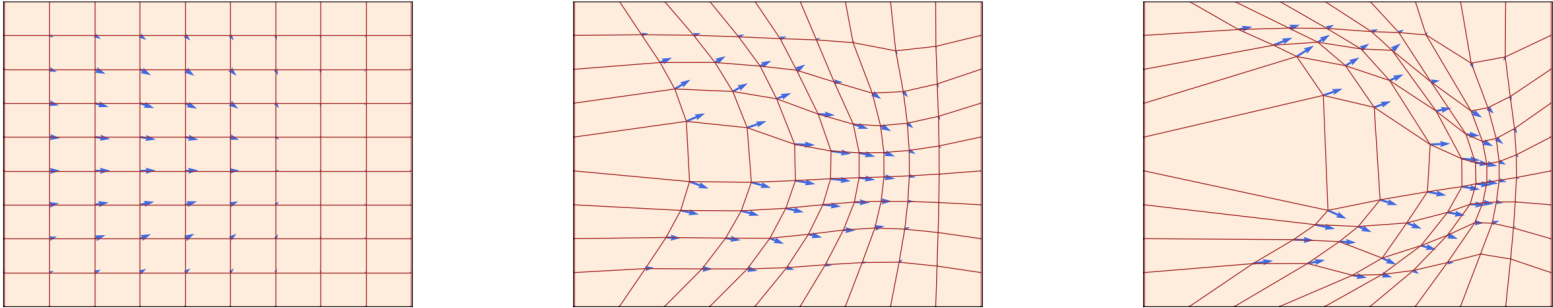
\includegraphics[width=\textwidth]{flow_example.png}
    \caption{Илюстрация на поток \(\psi_t : \mathbb{R}^d \rightarrow \mathbb{R}^d\), дефиниран чрез скоростно поле \(u_t : \mathbb{R}^d \rightarrow \mathbb{R}^d\). Червената квадратна решетка се деформира във времето, а сините стрелки показват локалните скорости. Фигурата визуализира как потокът ``изкривява'' пространството и реализира гладък пренос на проби \cite{lipman2024flowguide}.}
\end{figure}

Diffusion model разширява тази идея със стохастичен шумов член. В лекционните бележки SDE динамиката се записва като
\begin{equation}
d\mathbf{x}_t = \mathbf{v}(\mathbf{x}_t,t)\,dt + \sigma\,d\mathbf{W}_t,
\end{equation}
където \(\mathbf{v}\) е drift компонент, а \(d\mathbf{W}_t\) е броуново смущение \cite{mitnotes2026}. Същественото тук е, че според същите бележки ODE може да се разглежда като частен случай на SDE при \(\sigma_t=0\), тоест flow model и diffusion model принадлежат към една обща математическа рамка \cite{mitnotes2026}. За задачата по видео стабилизация това е полезна перспектива, защото позволява да се мисли за наблюдаваното движение като комбинация от структурна компонента и шумова компонента, която после се потиска чрез изглаждане.

Друга важна идея от съвременните diffusion models е score-based формулировката. Вместо моделът да учи директно траекторията, той може да учи score функцията \(\nabla \log p_t(\mathbf{x})\), която показва в коя посока трябва да се промени пробата, за да се придвижи към по-вероятни конфигурации \cite{song2021,mitnotes2026}. Лекционните бележки подчертават, че при Gaussian probability paths съществува директна връзка между векторното поле и score функцията, така че от едната величина може да се възстанови другата \cite{mitnotes2026}. Макар тази идея да не се използва директно в настоящата реализация, тя е важна теоретична отправна точка за разбирането защо съвременните генеративни модели работят чрез постепенна корекция на шумни състояния.

В рамките на настоящата курсова работа flow и diffusion models не се използват като практически стабилизиращи backend-и. Тяхната роля е по-скоро теоретична: те показват, че моделирането на движение, шум и еволюция във времето може да се формулира в общ език на ODE/SDE динамика. От тази гледна точка изглаждането на траектория в стабилизацията може да се разглежда като опростен инженерен аналог на идея, която в генеративните модели е развита много по-дълбоко и формално.

\subsection{Видео стабилизация}
Типичната стабилизираща верига се състои от три стъпки: оценка на междокадровото движение, изглаждане на траекторията на камерата и геометрично прехвърляне на кадрите към изгладена траектория. Ако \(\mathbf{p}_t\) е параметричният трансформ между кадрите, кумулативната траектория е
\begin{equation}
\mathbf{T}_t = \sum_{i=1}^{t}\mathbf{p}_i.
\end{equation}
След изглаждане се получава \(\widetilde{\mathbf{T}}_t\), а нужната корекция е
\begin{equation}
\mathbf{c}_t = \widetilde{\mathbf{T}}_t - \mathbf{T}_t.
\end{equation}
Колкото по-силно е изглаждането, толкова по-голяма е нуждата от crop или padding. Следователно стабилизацията винаги е компромис между устойчивост на картината и запазено зрително поле.

\section{Реализация}
В рамките на проекта беше реализиран офлайн стабилизатор в \texttt{stabilize.py}, който чете видеото кадър по кадър, оценява междокадровото движение, апроксимира глобален афинен модел чрез \texttt{RANSAC}, изглажда получената траектория и рендва стабилизирано видео. Системата поддържа два backend-а за движение, обозначени като \texttt{lk} и \texttt{raft}, като и двата използват обща стабилизираща логика след етапа на оценка на движението. По този начин сравнението между тях не е сравнение на две различни стабилизиращи системи, а сравнение на две различни стратегии за оценка на движението в една и съща pipeline структура.

Глобалното движение на камерата се моделира чрез частичен афинен трансформ. Това решение беше избрано като компромис между изразителност и устойчивост. То е по-гъвкаво от чиста транслация и в същото време по-стабилно и по-интерпретируемо от пълна хомография за настоящите експериментални сценарии. Върху получената траектория бяха реализирани два типа изглаждане: moving average и EMA. След отстраняване на ранни логически грешки в стабилизиращата математика беше въведен и параметър \texttt{correction\_strength}, който позволява частично прилагане на корекцията и намалява риска от свръхкомпенсация при по-слабо трептене.

Особено важен момент в реализацията е начинът на оценка на качеството. Вместо да се разчита само на вътрешните трансформи, системата извършва втори проход върху финалното стабилизирано видео и измерва остатъчното движение в готовия резултат. Това дава значително по-честна метрика, защото именно крайното видео е реалният обект на оценка.

\section{Експериментална постановка}
В работата бяха използвани няколко клипа с различна роля. Основният положителен benchmark е \texttt{car\_input\_20s.mp4}, тъй като при него камерата действително има изразено нежелано движение и ефектът от стабилизацията може да се измери ясно. Клипът \texttt{piano\_input.mp4} служи като по-лек сценарий, при който движението е по-слабо и съответно ефектът от стабилизацията е по-умерен. Видеото \texttt{crowd.mp4} беше използвано като неуспешен сценарий, защото съдържа предимно движение на обекти при почти статична камера.

За количествена оценка се използват ratio метрики върху стандартното отклонение на остатъчното движение по двете оси, ratio за ротационния jitter, скоростта на оценка на движението в кадри за секунда и относителният запазен зрителен ъгъл след crop. При ratio под \(1\) стабилизацията е полезна, защото остатъчното движение в изхода е по-малко от това във входното видео.

В основното параметрично изследване за LK бяха разгледани стойности \texttt{smooth\_radius} от 15 и 30, както и \texttt{correction\_strength} от 0.6, 0.8 и 1.0. След намиране на най-добрата настройка беше проведено изследване на устойчивостта при контролирани деградации на \texttt{car\_input\_20s.mp4}, включително H.264 рекомпресия, Gaussian blur и downscale.

\section{Резултати}
Първият важен резултат е, че за основния клип \texttt{car\_input\_20s.mp4} най-добрата конфигурация използва backend \texttt{lk}, изглаждане с moving average, \texttt{smooth\_radius}=30 и \texttt{correction\_strength}=1.0. При тази настройка са получени \(\texttt{ratio\_x}=0.555\) и \(\texttt{ratio\_y}=0.145\), което означава приблизително \(44.5\%\) намаление на остатъчното движение по хоризонталната ос и \(85.5\%\) по вертикалната. Това е силен положителен резултат и показва, че стабилизацията е не само визуално убедителна, но и количествено измерима.

\begin{figure}[H]
    \centering
    \begin{minipage}[t]{0.49\textwidth}
        \vspace{0pt}
        \centering
        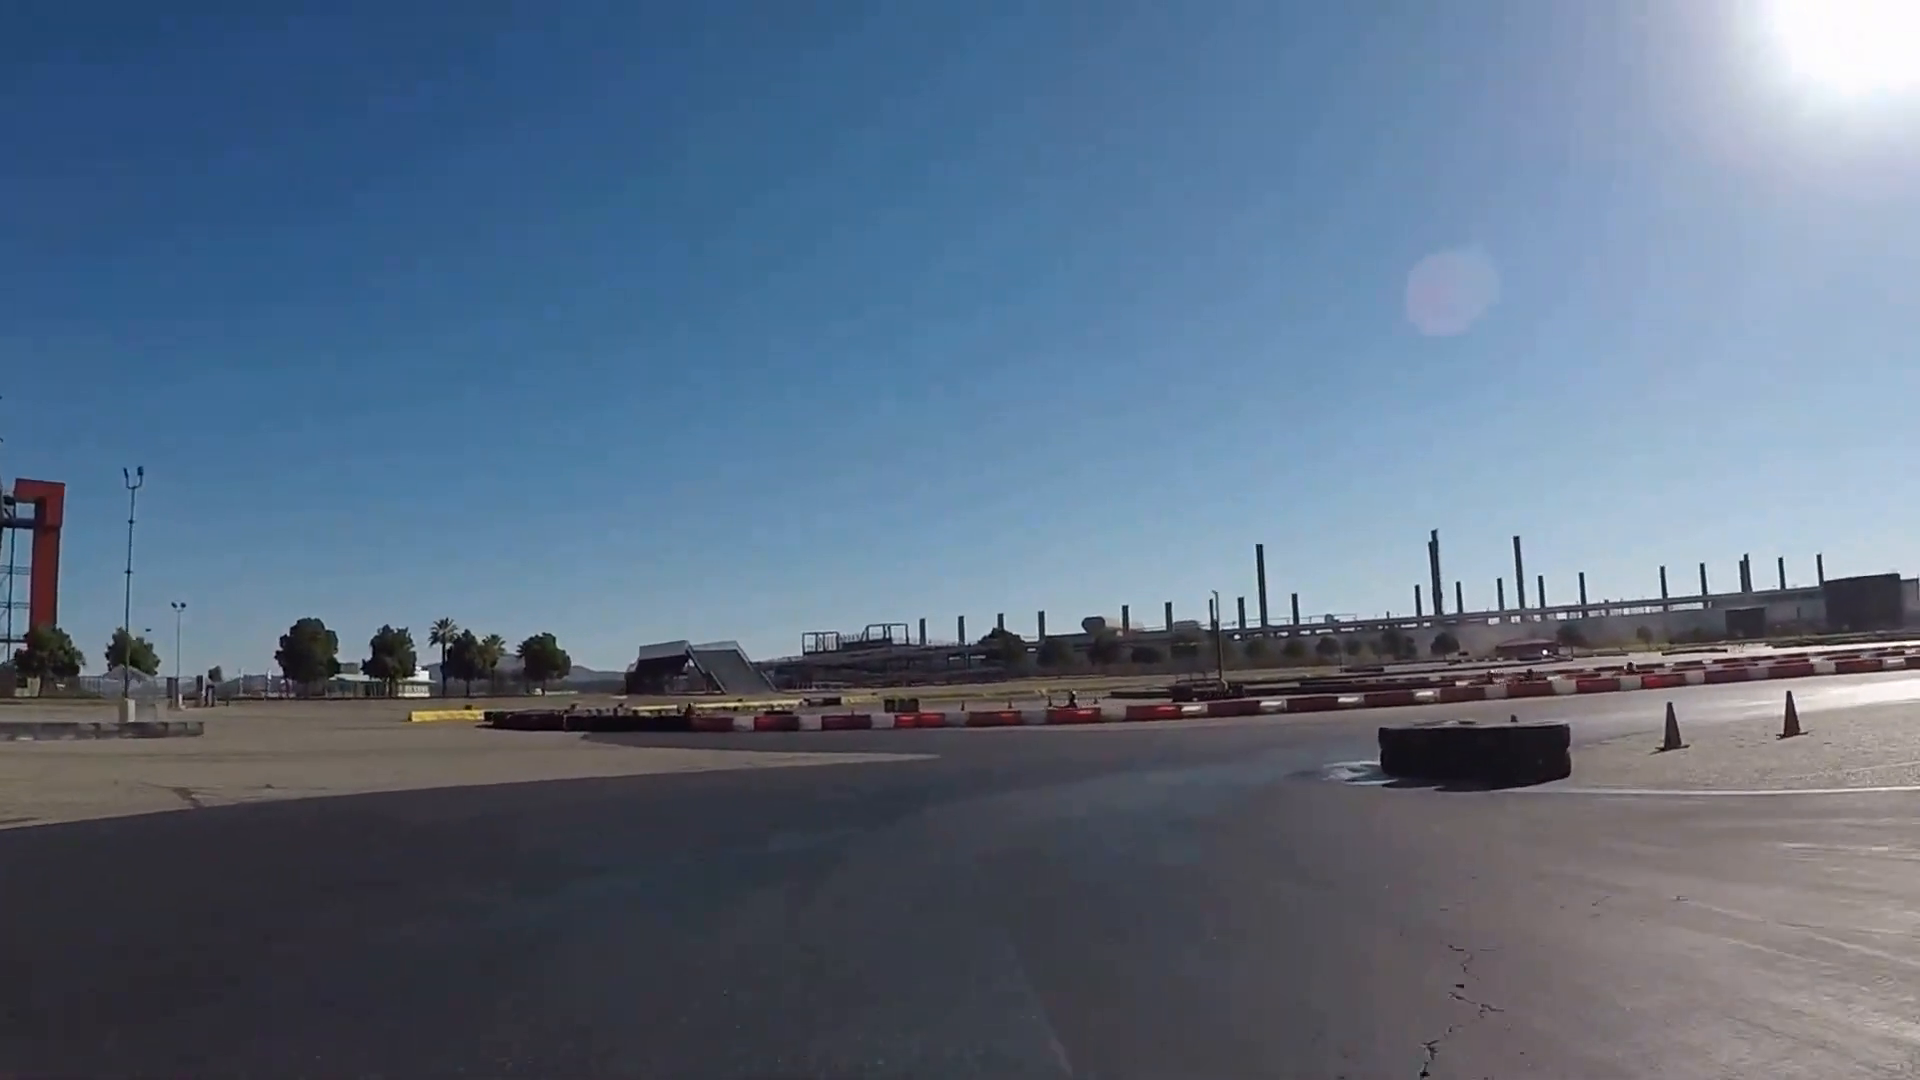
\includegraphics[width=\linewidth]{car_input_20s_frame.png}\\[0.3em]
        \small Входен кадър от \texttt{car\_input\_20s.mp4}
    \end{minipage}\hfill
    \begin{minipage}[t]{0.49\textwidth}
        \vspace{0pt}
        \centering
        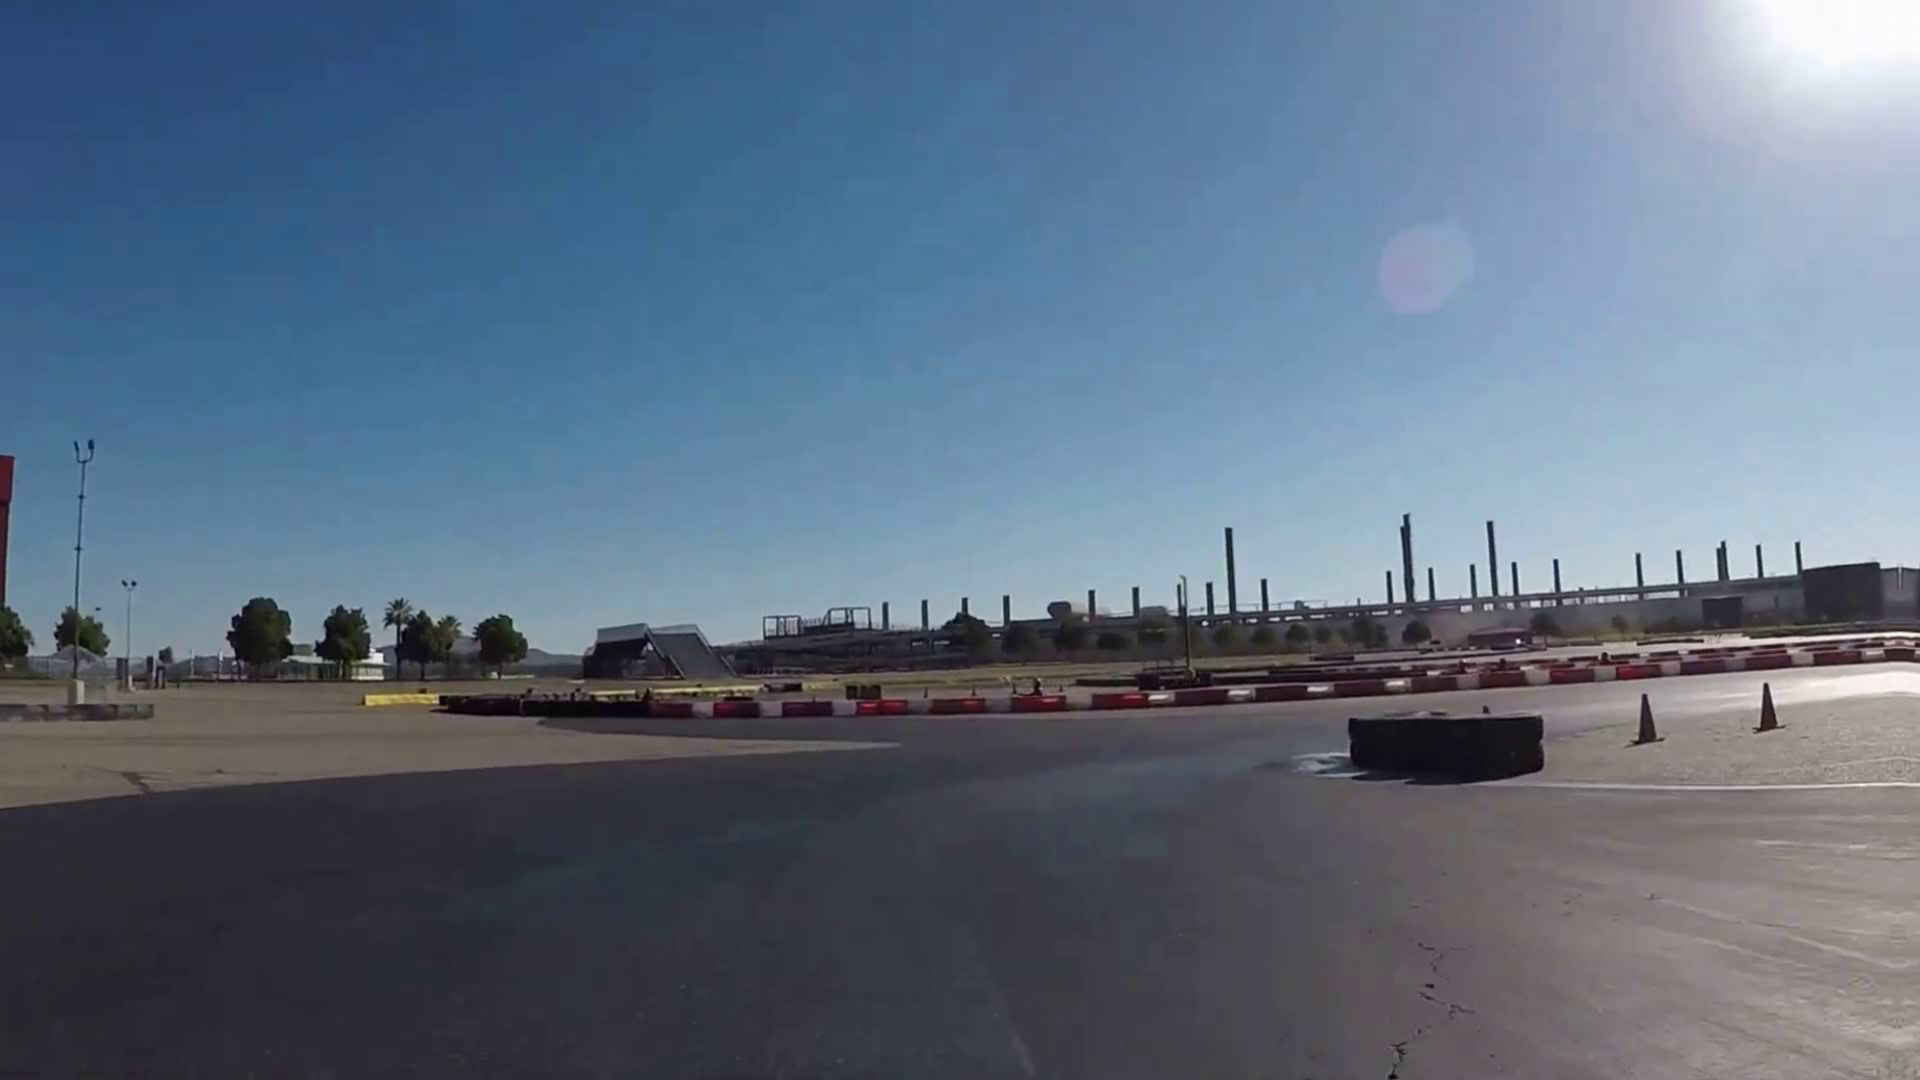
\includegraphics[width=\linewidth]{car_input_20s_lk_best_frame.png}\\[0.3em]
        \small Кадър от стабилизирания резултат при най-добрата LK настройка
    \end{minipage}
    \caption{Репрезентативен кадър около десетата секунда от основния автомобилен benchmark преди и след стабилизация. Единичният кадър не показва цялата динамика на трептенето, но визуализира запазването на сцената и умерения crop при финалния резултат.}
\end{figure}

За същата най-добра конфигурация се наблюдава и силно потискане на ротационното трептене: \(\texttt{ratio\_rot}=0.114\), тоест приблизително \(88.6\%\) редукция на ротационния jitter. Допълнително \(\texttt{valid\_fov\_ratio\_after\_crop}=0.943\), което означава, че след прилагане на \texttt{crop\_margin}=20 системата запазва около \(94.3\%\) от първоначалното зрително поле. Това е практически важен резултат, защото показва, че силната стабилизация не е постигната с прекомерна загуба на полезно изображение.

\begin{table}[H]
    \centering
    \caption{Обобщение на най-добрата конфигурация за \texttt{car\_input\_20s.mp4}}
    \begin{tabular}{ccccc}
        \toprule
        Ratio \(x\) & Ratio \(y\) & Ratio rot & FPS & Запазено FOV \\
        \midrule
        0.555 & 0.145 & 0.114 & 25.23 & 0.943 \\
        \bottomrule
    \end{tabular}
\end{table}

\begin{table}[H]
    \centering
    \caption{Параметричен sweep за LK върху \texttt{car\_input\_20s.mp4}}
    \begin{tabular}{cccccc}
        \toprule
        Метод & Radius & Strength & Ratio \(x\) & Ratio \(y\) & FPS \\
        \midrule
        LK & 15 & 0.6 & 0.666 & 0.409 & 26.90 \\
        LK & 15 & 0.8 & 0.617 & 0.241 & 25.38 \\
        LK & 15 & 1.0 & 0.586 & 0.163 & 24.87 \\
        LK & 30 & 0.6 & 0.684 & 0.405 & 25.05 \\
        LK & 30 & 0.8 & 0.576 & 0.233 & 24.11 \\
        LK & 30 & 1.0 & \textbf{0.555} & \textbf{0.145} & 25.23 \\
        \bottomrule
    \end{tabular}
\end{table}

\begin{figure}[H]
    \centering
    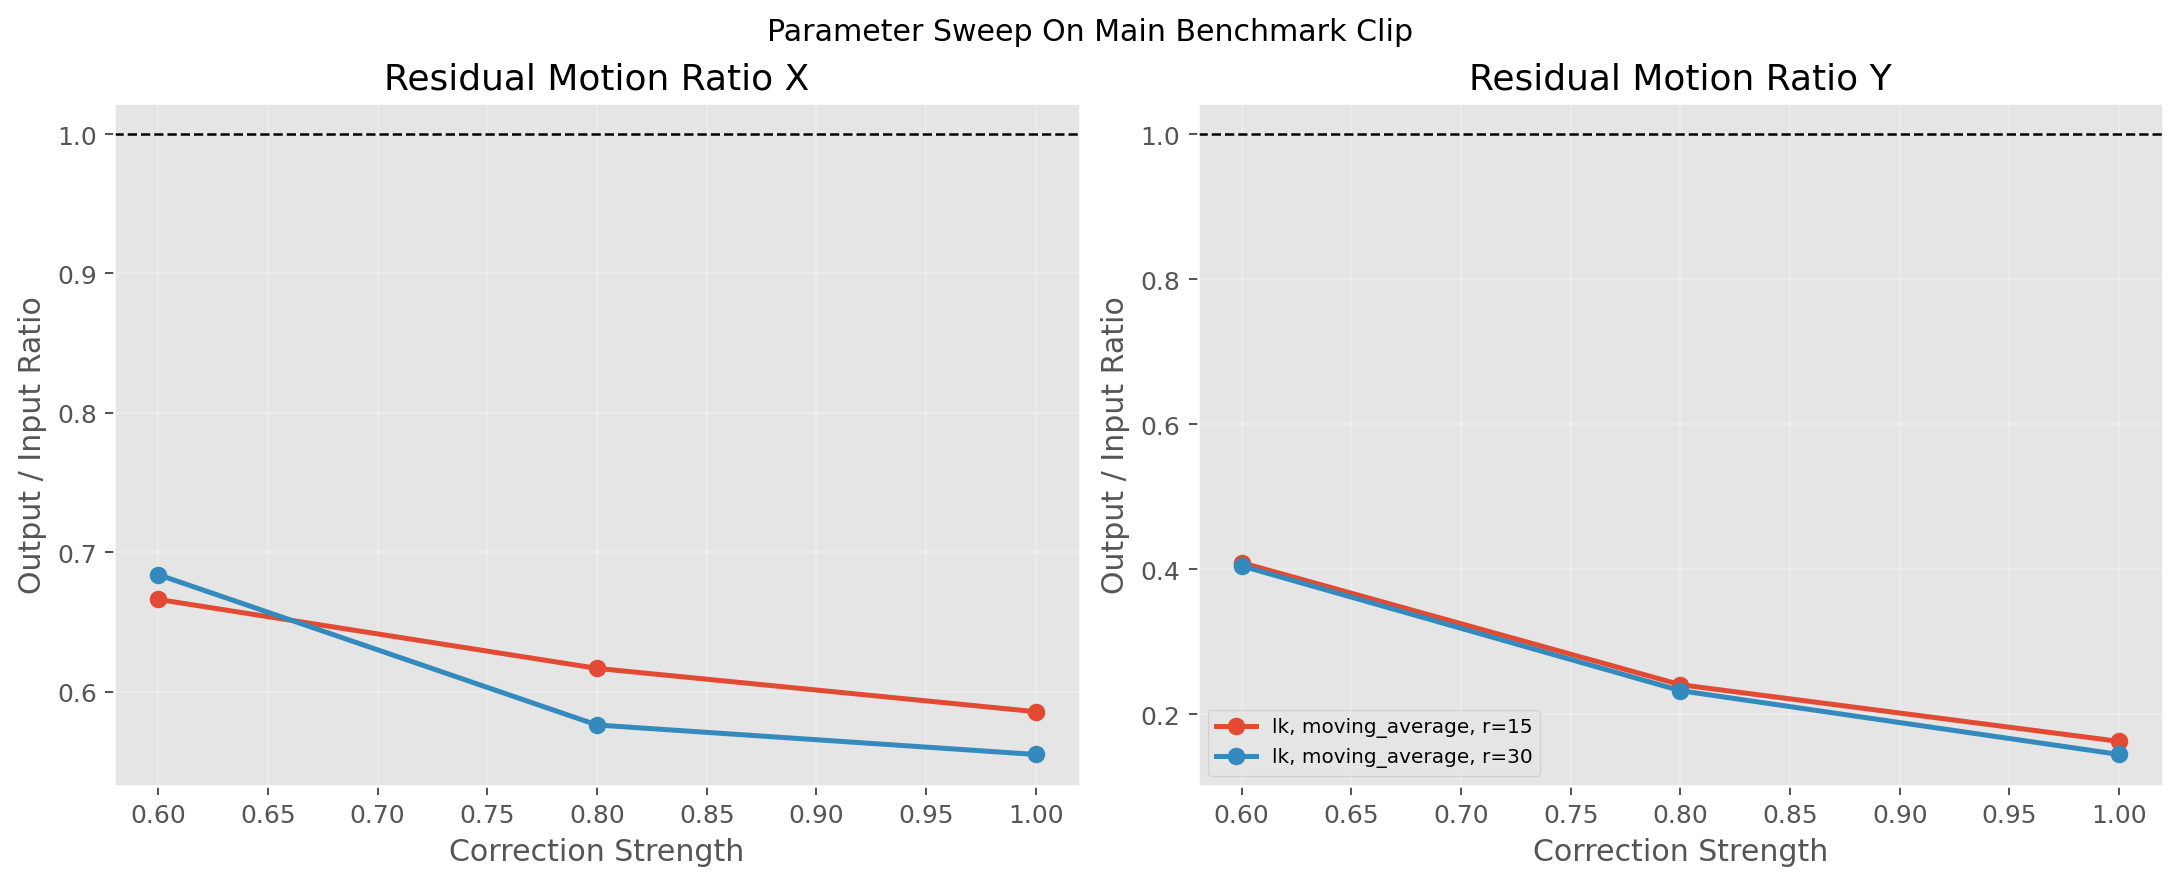
\includegraphics[width=0.92\textwidth]{parameter_sweep_ratios.png}
    \caption{Влияние на \texttt{smooth\_radius} и \texttt{correction\_strength} върху остатъчното движение.}
\end{figure}

Фигурата и таблицата показват ясна тенденция: за този клип по-силната корекция работи по-добре, а по-големият радиус на изглаждане дава по-стабилна траектория. Това е показателно, защото при реални системи често се приема, че агресивното изглаждане задължително води до лош визуален компромис, но в конкретния случай то се оказва най-ефективната настройка.

Като вторични наблюдения могат да се посочат още два полезни сценария. При \texttt{piano\_input.mp4} стабилизацията остава полезна, но ефектът е по-умерен: за най-добрия наличен LK резултат са отчетени \((0.795, 0.659)\) по осите, \(\texttt{ratio\_rot}=0.614\), около \(110.8\) FPS и \(\texttt{valid\_fov\_ratio}=0.874\). Това е очаквано, защото входното трептене е с по-малка амплитуда и съответно има по-малко пространство за подобрение. Обратно, \texttt{crowd.mp4} е показателен неуспешен сценарий: при почти статична камера и доминиращо движение на хора измерените стойности след стабилизацията се влошават спрямо входа, а запазеното зрително поле спада до \(0.833\). Така двата допълнителни клипа допълват основния автомобилен benchmark, но не променят централния извод, че \texttt{car\_input\_20s.mp4} е най-силният и най-показателен положителен пример в настоящата работа.

\begin{table}[H]
    \centering
    \caption{Допълнителни резултати за \texttt{piano\_input.mp4} и \texttt{crowd.mp4}}
    \begin{tabular}{lccccc}
        \toprule
        Видео / настройка & Ratio \(x\) & Ratio \(y\) & Ratio rot & FPS & FOV \\
        \midrule
        Piano, LK, cs=0.8 & 0.794 & 0.780 & 0.678 & 115.11 & 0.874 \\
        Piano, LK, cs=1.0 & 0.795 & 0.659 & 0.614 & 110.83 & 0.874 \\
        Crowd, RAFT & 2.223 & 2.698 & 1.720 & 13.71 & 0.833 \\
        \bottomrule
    \end{tabular}
\end{table}

\begin{figure}[H]
    \centering
    \begin{minipage}[t]{0.49\textwidth}
        \vspace{0pt}
        \centering
        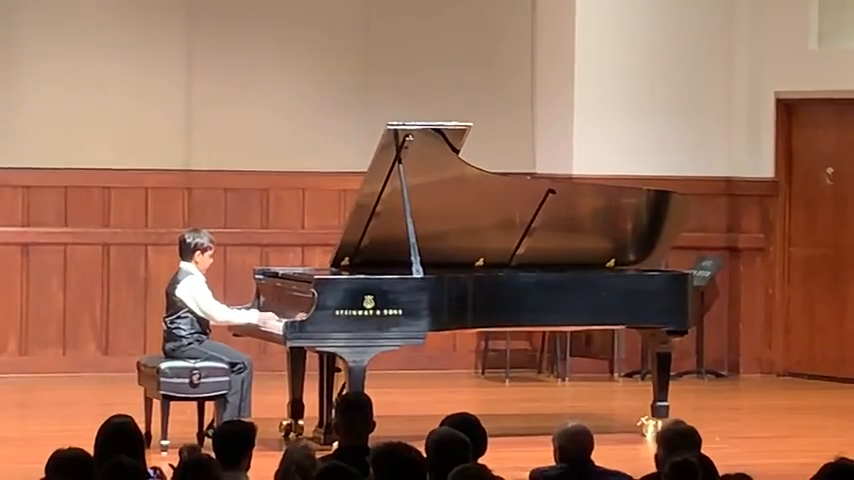
\includegraphics[width=\linewidth]{piano_input_frame.png}\\[0.3em]
        \small Кадър от \texttt{piano\_input.mp4}
    \end{minipage}\hfill
    \begin{minipage}[t]{0.49\textwidth}
        \vspace{0pt}
        \centering
        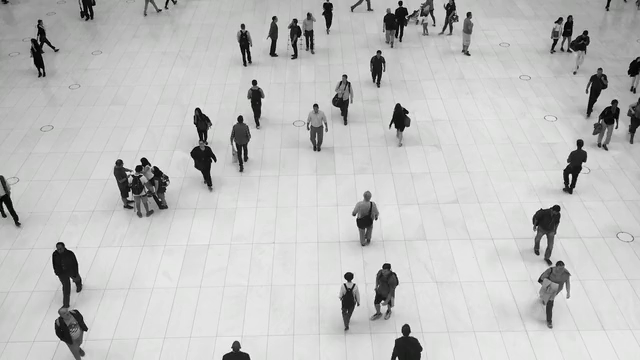
\includegraphics[width=\linewidth]{crowd_input_frame.png}\\[0.3em]
        \small Кадър от \texttt{crowd.mp4}
    \end{minipage}
    \caption{Двата вторични сценария в работата. \texttt{piano\_input.mp4} е пример за по-слабо входно трептене, при което стабилизацията е полезна, но умерена, докато \texttt{crowd.mp4} е труден случай, в който независимо движещите се хора нарушават оценката на глобалното движение на камерата.}
\end{figure}

Втората голяма група експерименти анализира устойчивостта на най-добрата LK конфигурация при различни деградации. Резултатите показват, че H.264 компресията има сравнително ограничено влияние: дори при CRF 35 стойностите остават около \((0.564, 0.161)\). Blur също не разрушава стабилизацията и двете разгледани степени на замъгляване водят до близки стойности около \((0.55, 0.14)\). Най-осезаемо влияние има downscale, особено при \(0.5\times\), но дори тогава стабилизацията остава силна и осигурява ratios \((0.612, 0.163)\), като в замяна скоростта на обработка нараства значително.

\begin{table}[H]
    \centering
    \caption{Устойчивост на най-добрата LK конфигурация при деградации на \texttt{car\_input\_20s.mp4}}
    \begin{tabular}{lcccc}
        \toprule
        Деградация & Параметър & Ratio \(x\) & Ratio \(y\) & FPS \\
        \midrule
        H.264 & CRF 23 & 0.549 & 0.152 & 26.09 \\
        H.264 & CRF 28 & 0.550 & 0.143 & 26.03 \\
        H.264 & CRF 35 & 0.564 & 0.161 & 25.90 \\
        Blur & \(\sigma = 1.5\) & 0.549 & 0.139 & 25.61 \\
        Blur & \(\sigma = 3.0\) & 0.552 & 0.145 & 26.23 \\
        Downscale & \(0.75\times\) & 0.605 & 0.149 & 40.85 \\
        Downscale & \(0.5\times\) & 0.612 & 0.163 & 87.09 \\
        \bottomrule
    \end{tabular}
\end{table}

\begin{figure}[H]
    \centering
    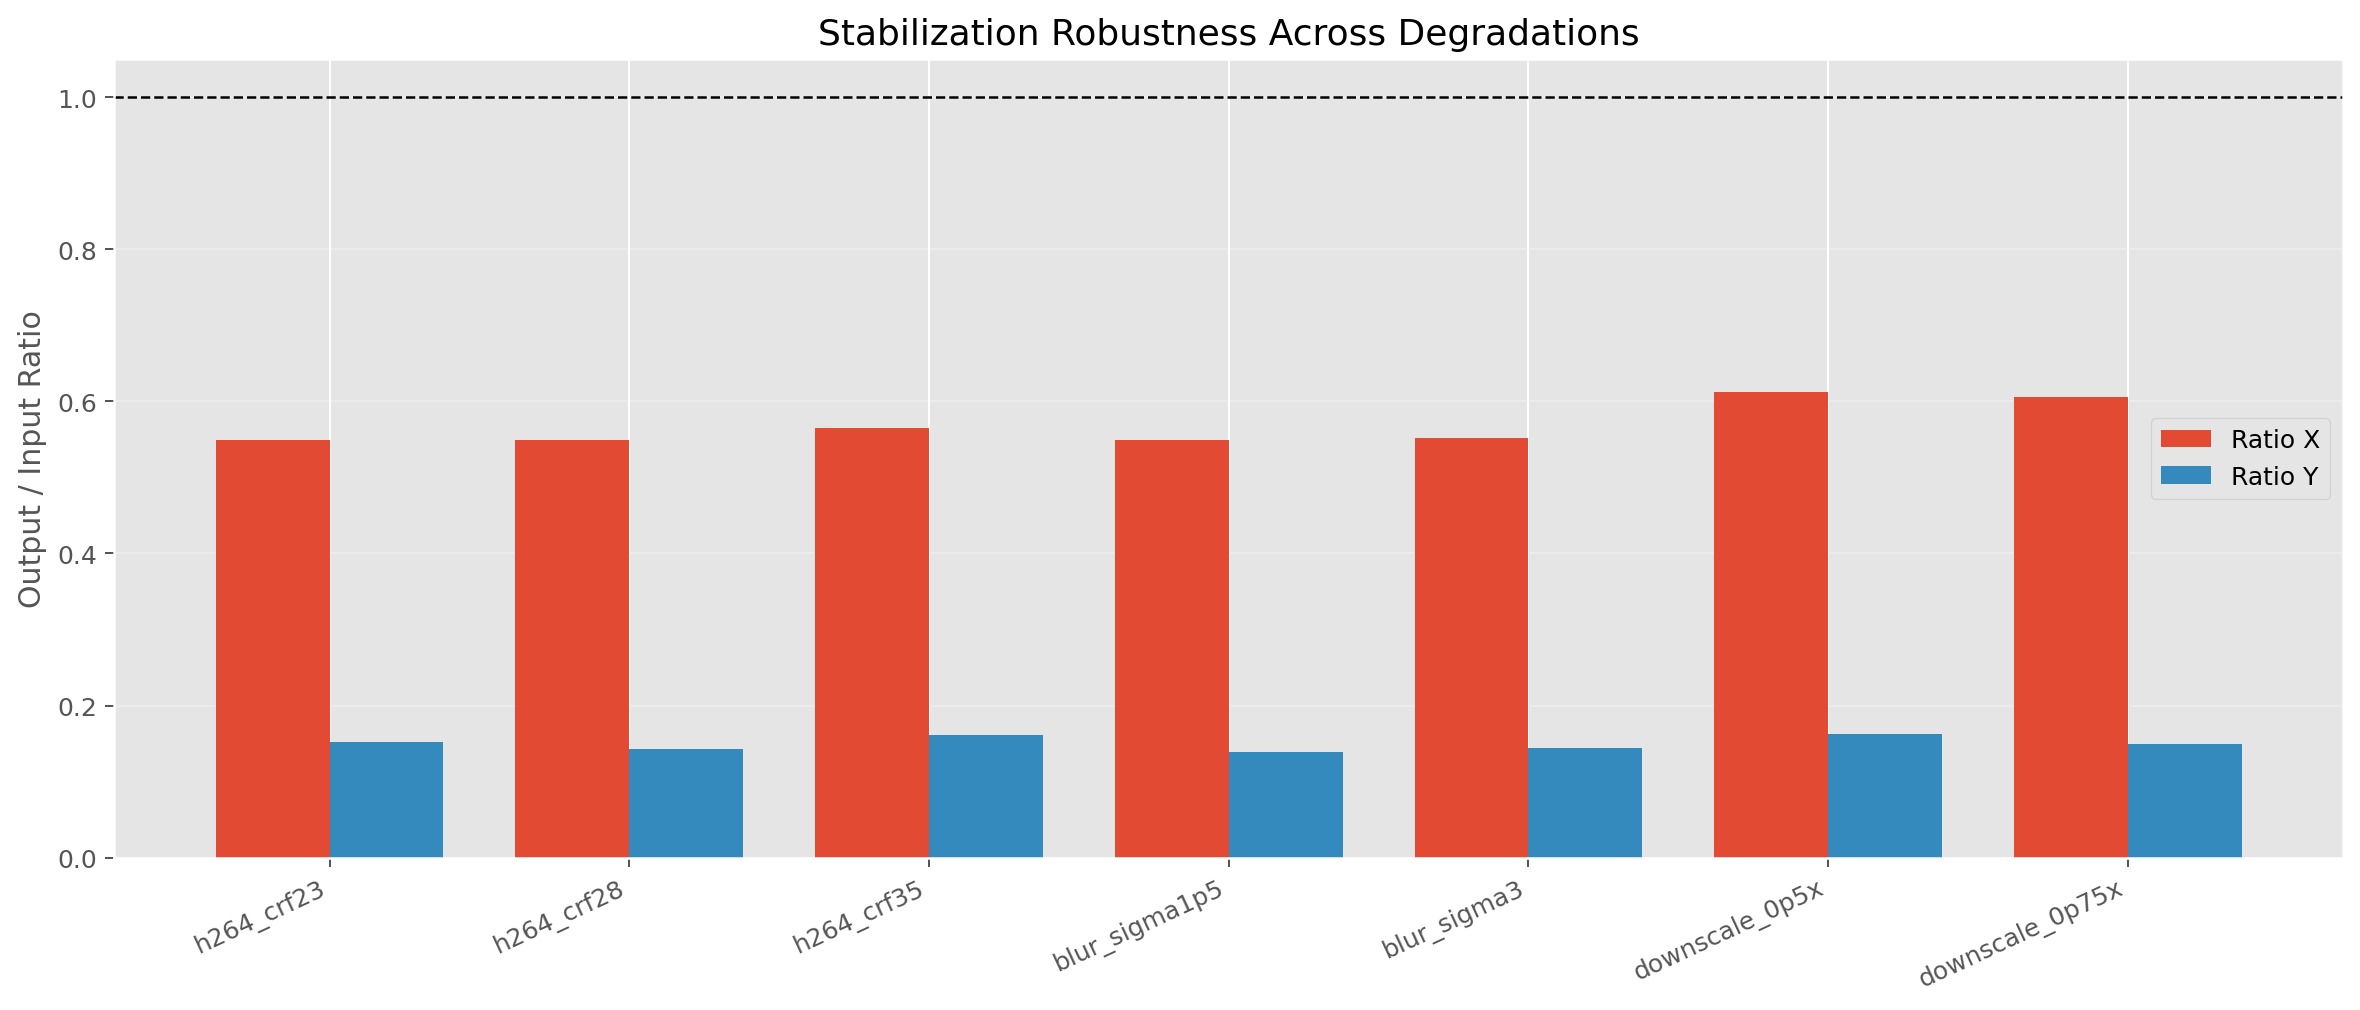
\includegraphics[width=0.95\textwidth]{degradation_ratios.png}
    \caption{Остатъчни ratio стойности при различните деградации.}
\end{figure}

\begin{figure}[H]
    \centering
    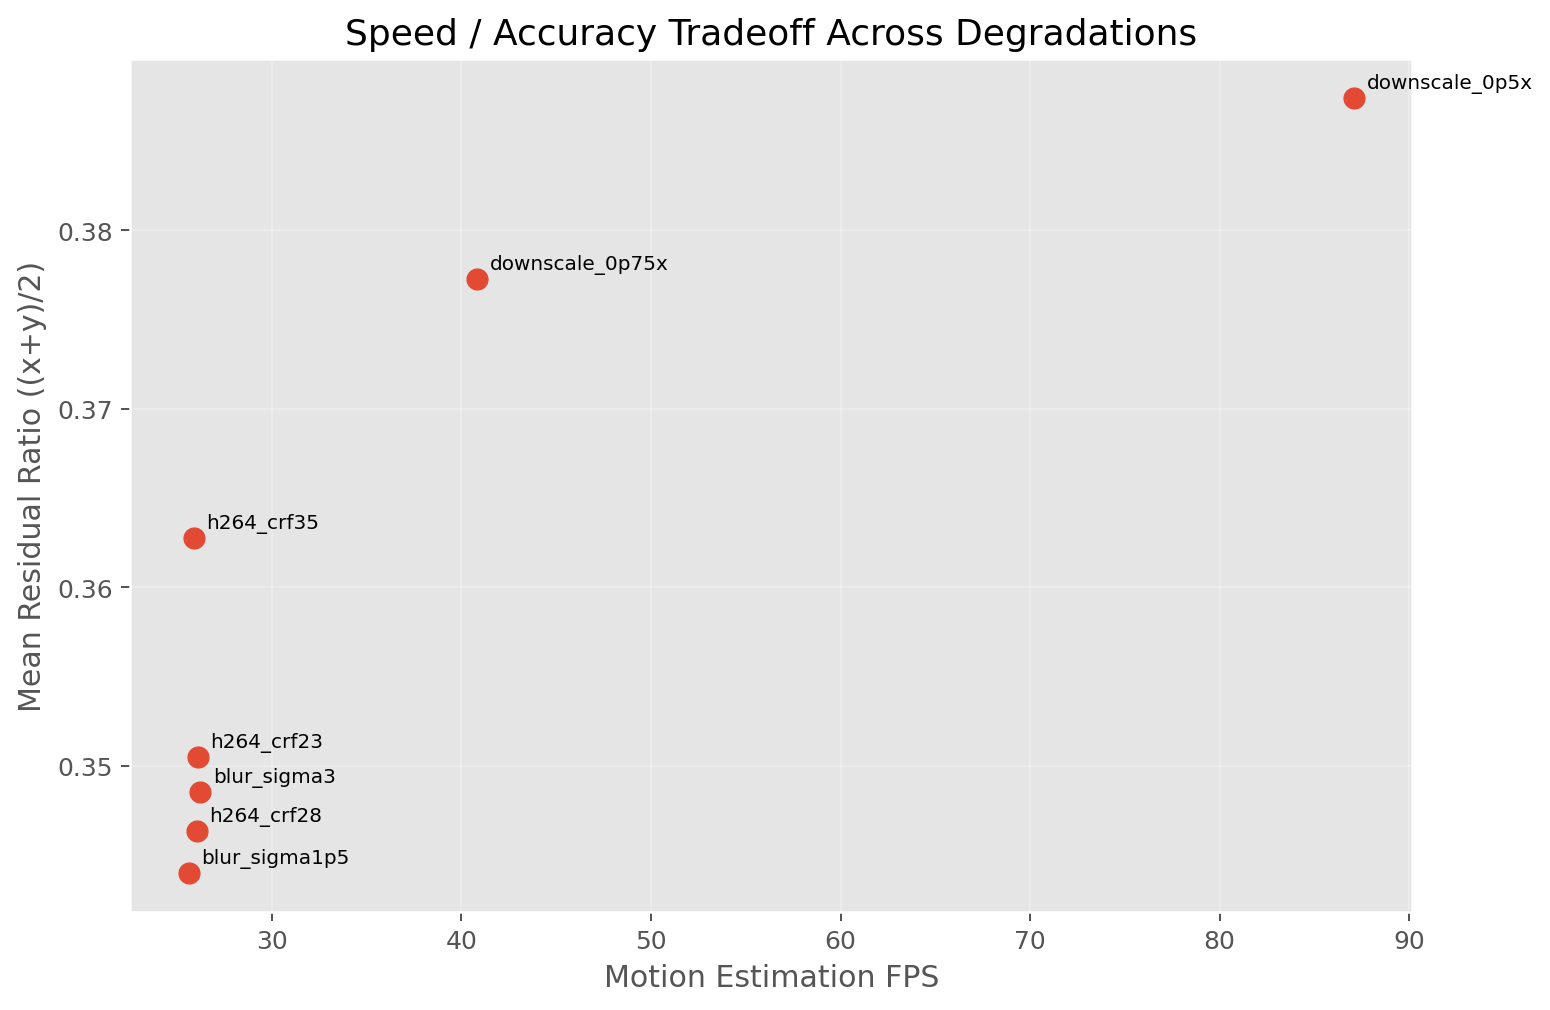
\includegraphics[width=0.84\textwidth]{degradation_speed_tradeoff.png}
    \caption{Компромис между точност и скорост при различните деградации.}
\end{figure}

Този резултат е важен и от практическа гледна точка. Той показва, че системата не е крехка спрямо често срещани мултимедийни трансформации. Компресията и умереното замъгляване не я разрушават, а downscale създава добре изразен компромис между точност и производителност, който може да бъде полезен в реални приложения.

Третият важен резултат е backend сравнението между LK и RAFT. На пълната резолюция на \texttt{car\_input\_20s.mp4} RAFT не можа да бъде използван върху наличния хардуер поради недостиг на GPU памет. Това не е просто технически неуспех, а реален експериментален извод: силният дълбок оптичен поток може да бъде трудно приложим за стабилизация при ограничени ресурси. За да се направи все пак честно сравнение, беше използван downscale \(0.5\times\) вариант на същия клип и RAFT-small. Там RAFT-small постигна \((0.744, 0.696)\) при около 22 FPS, докато LK върху същия \(0.5\times\) вход постигна \((0.612, 0.163)\) при около 87 FPS. Следователно в рамките на тази реализация LK е не само по-бърз, но и по-ефективен като стабилизиращ backend.

\section{Обсъждане}
Получените резултати подкрепят тезата, че за видео стабилизация най-важна не е детайлността на локалното поле на движение, а надеждността, с която може да бъде извлечено едно глобално движение на камерата. Именно тук Lucas--Kanade има естествено предимство. Той работи със сравнително малък, но стабилен набор от точки, от които глобалният афинен модел се извлича по-пряко. При RAFT ситуацията е обратна: получава се богат плътен поток, но редукцията му до един глобален трансформ е трудна и чувствителна към движение на обекти в сцената.

Това обяснява и защо сцената с \texttt{crowd.mp4} е толкова показателна. При почти статична камера и голям брой движещи се хора системата наблюдава много локално движение, което обаче не е движение на камерата. Следователно подобни сцени са естествена граница за текущия подход. Същевременно основният автомобилен клип показва обратния случай: когато доминиращото движение наистина идва от камерата, стабилизацията е силна и надеждна.

Оттук следва и по-общият инженерен извод. В настоящия проект плътният optical flow не се оказа оптималният инструмент за глобална стабилизация, въпреки теоретичната си сила. Това не означава, че дълбоките модели са безполезни, а че задачата по стабилизация има различен оптимум от задачата по общ optical flow benchmarking. Практическата стойност на даден модел се определя от цялата pipeline, а не само от локалната му точност.

\section{Ограничения и бъдеща работа}
Основното ограничение на настоящата работа е, че положителният benchmark се базира на ограничен брой клипове, като най-силен и добре анализиран е \texttt{car\_input\_20s.mp4}. Освен това transformer baseline от типа GMFlow или FlowFormer не е реализиран в пълен вид. От експериментална гледна точка това е разбираемо, защото дори RAFT на пълна резолюция се оказа непрактичен върху наличния хардуер, но все пак остава ограничение спрямо първоначално по-широката идея за сравнение.

Естествените посоки за бъдеща работа включват по-добра селекция на фон, използване на маски за движещи се обекти, ограничено сравнение с transformer модел в по-ниска резолюция, както и евентуално сравнение между афинен модел и хомография. Полезно продължение би било и автоматизирано генериране на финални фигури и таблици за директно включване в окончателния отчет.

\section{Заключение}
В тази курсова работа беше разработена и изследвана система за видео стабилизация чрез оценяване на междокадровото движение и изглаждане на траекторията на камерата. Бяха реализирани два backend-а --- Lucas--Kanade и RAFT --- и беше проведено систематично сравнение между тях в една и съща стабилизираща верига. Получените резултати показват, че в разглеждания практически контекст Lucas--Kanade е по-добрият избор. Той дава едновременно висока стабилизационна ефективност, добра скорост и по-ниска хардуерна цена.

Най-добрият резултат върху основния benchmark \texttt{car\_input\_20s.mp4} е \((0.555, 0.145)\), което показва силно намаляване на остатъчното движение. Освен това системата остава устойчива при компресия, blur и downscale. Сравнението с RAFT-small върху намалена резолюция допълнително потвърждава, че по-точният плътен поток не е достатъчен, ако не може надеждно да бъде превърнат в стабилен глобален модел на камерата. Следователно основният принос на работата е не само в реализирания код, а и в експериментално аргументирания извод, че за тази задача класическият sparse подход е по-практичен от тежкия deep optical flow backend.

Изходният код, LaTeX източникът на отчета и допълнителните демонстрационни материали са публикувани в GitHub хранилището на проекта: \url{https://github.com/Apsie09/Video-Stabilization-Optical-Flow-RAFT}.

\begin{thebibliography}{99}

\bibitem{horn1981}
Horn, B. K. P., Schunck, B. G.
\newblock Determining Optical Flow.
\newblock \emph{Artificial Intelligence}, 17(1--3), 185--203, 1981.

\bibitem{lucaskanade1981}
Lucas, B. D., Kanade, T.
\newblock An Iterative Image Registration Technique with an Application to Stereo Vision.
\newblock In \emph{Proceedings of Imaging Understanding Workshop}, 121--130, 1981.

\bibitem{raft2020}
Teed, Z., Deng, J.
\newblock RAFT: Recurrent All-Pairs Field Transforms for Optical Flow.
\newblock In \emph{Proceedings of ECCV}, 402--419, 2020.

\bibitem{ho2020}
Ho, J., Jain, A., Abbeel, P.
\newblock Denoising Diffusion Probabilistic Models.
\newblock In \emph{Proceedings of NeurIPS}, 2020.

\bibitem{song2021}
Song, Y., Sohl-Dickstein, J., Kingma, D. P., Kumar, A., Ermon, S., Poole, B.
\newblock Score-Based Generative Modeling through Stochastic Differential Equations.
\newblock In \emph{Proceedings of ICLR}, 2021.

\bibitem{mitcourse2026}
MIT 6.S184 Course Website.
\newblock \emph{Introduction to Flow Matching and Diffusion Models}, 2026.
\newblock \url{https://diffusion.csail.mit.edu/2026/index.html}

\bibitem{mitnotes2026}
Holderrieth, P., Erives, E.
\newblock \emph{An Introduction to Flow Matching and Diffusion Models}.
\newblock MIT Class 6.S184 Lecture Notes, 2026.
\newblock \url{https://diffusion.csail.mit.edu/2026/docs/lecture_notes.pdf}

\bibitem{lipman2024flowguide}
Lipman, Y., Havasi, M., Holderrieth, P., Shaul, N., Le, M., Karrer, B., Chen, R. T. Q., Lopez-Paz, D., Ben-Hamu, H., Gat, I.
\newblock \emph{Flow Matching Guide and Code}.
\newblock arXiv:2412.06264, 2024.
\newblock \url{https://arxiv.org/abs/2412.06264}

\bibitem{opencvdocs}
OpenCV Documentation.
\newblock Lucas--Kanade Optical Flow and Geometric Transform Estimation.
\newblock \url{https://opencv.org/}

\end{thebibliography}

\end{document}
